\chapter*{Introducci\'on}
\addcontentsline{toc}{chapter}{Introducci\'on}

  El desarrollo de software se encuentra en una transici\'on de paradigmas 
  de programaci\'on,  tal como a\~nos
  atr\'as se di\'o cuando  la programaci\'on estructurada fu\'e reemplazada 
  por la programaci\'on orientada a objetos \citep{roadStructuredToOO}. En este caso la siguiente  
  etapa que esta sentando presencia es la de programaci\'on funcional.
\\
\\  
  Como consecuencia del uso extensivo del paradigma orientado a objetos
  el uso de t\'ecnicas y tecnolog\'ias diferentes tiene un grado de dificultad
  adicional. Tal situaci\'on representa un gran problema 
  para el  \'area de desarrollo de software ya que las tendencias actuales 
  forzar\'an a un cambio de paradigma y conceptos de desarrollo 
  que afectar\'an a la industria, tanto por los problemas de adopci\'on
  como por los problemas inherentes a cualquier cambio de tecnolog\'ia.
\\ 
\\ 
  Esta situaci\'on est\'a forzando a que las empresas de desarrollo tomen en cuenta a la 
  transici\'on de forma paulatina, reduciendo costos y aumentando al m\'aximo
  el retorno de inversi\'on.

\section*{Definici\'on del problema}
\addcontentsline{toc}{section}{Definici\'on del problema}
  
  La reciente popularidad de los lenguajes de programaci\'on funcionales
  conllevar\'an al aumento del desarrollo de plataformas y oportunidades de mercado 
  para tales lenguajes \citep{scalaPotentialUk}. De la misma forma que el paradigma orientado a 
  objetos forz\'o un cambio en la industria en la d\'ecada de los sesenta  \citep{roadStructuredToOO}.
\\ 
\\
  Tal situaci\'on es conocida por las empresas de desarrollo y se marca
  una tendencia en la industria orient\'andola hacia la
  programaci\'on funcional, ya que este tipo de programaci\'on est\'a
  enfocada a resolver muchos de los problemas existentes tanto en 
  la programaci\'on estructurada como en la programaci\'on orientada 
  a objetos.
\\ 
\\ 
  Pero el paradigma de programaci\'on funcional es diferente y puede
  tener una curva de aprendizaje elevada para desarrolladores que
  vienen desde un enfoque orientado a objetos. Para resolver este
  problema se han creado lenguajes mixtos que incluyen los aspectos
  de la programaci\'on orientada a objetos y las bondades de la
  programaci\'on funcional. El lenguaje predominante dentro de esta
  categor\'ia, tanto en la industria como acad\'emicamente es
  Scala\citep{scalaIntro}.
\\ 
\\ 
  Adicionalmente a este problema existen los problemas de
  escalabilidad de las aplicaciones debido a la arquitectura que
  utilizan.  En la industria de desarrollo existe un movimiento
  iniciado por Trygve Reenskaug\footnote{Creador del patr\'on de
    dise\~no MVC} que retoma a la arquitectura de sistemas como base
  de todo desarrollo escalable de aplicaciones.
\\ 
\\
  Seg\'un Reenskaug las plataformas de desarrollo actuales que est\'an
  basadas en el patr\'on de dise\~no \gls{MVC} como arquitectura de sistemas
  tienen un enfoque err\'oneo, ya que \gls{MVC} fu\'e concebida como una
  t\'ecnica de representaci\'on de datos y no as\'i una arquitectura
  de sistema \citep{dciIntro}. Las consecuencias de usar \gls{MVC} como arquitectura 
  del sistema han generado problemas de escalabilidad ya que nunca estuvo 
  orientada a cubrir este tipo de problemas, tal es el caso de Twitter 
  la cual reemplaz\'o su sistema base \gls{MVC} en Rails por un sistema personalizado 
  escrito en Scala \citep{twitterScala}. Y tales problemas tienen incidencia en 
  la velocidad de desarrollo en un sistema ya existente, retrasando la inclusi\'on 
  de nuevas caracter\'isticas y el arreglo de errores de forma r\'apida 
  \citep{codeReadability}.
\\
\\
  La propuesta de Reenskaug es la arquitectura \gls{DCI} \citep{dciIntro}
  ,la cual define una
  estructura de aplicaci\'on en la que el dominio del negocio de la
  misma se representa a trav\'es de componentes espec\'ificos con
  responsabilidades definidas. Esta arquitectura utiliza conceptos y
  facilidades de lenguajes funcionales combinados con los conceptos de
  orientaci\'on a objetos.
\\
\\
  Pero la implementaci\'on de tal arquitectura requiere de caracter\'isticas
  espec\'ificas en los lenguajes de programaci\'on, como ser la herencia 
  m\'ultiple y la composici\'on de componentes en tiempo de ejecuci\'on (\gls{mixin}) 
  \citep{dciIntro}.

\section*{Situaci\'on problem\'atica}
\addcontentsline{toc}{section}{Situaci\'on problem\'atica}

  La falta de un enfoque arquitect\'onico orientado a la escalabilidad de sistemas en las
  plataformas de desarrollo empresariales dificulta la creaci\'on y mantenimiento 
  de aplicaciones incrementando la complejidad de las mismas. 

\section*{Situaci\'on deseada}
\addcontentsline{toc}{section}{Situaci\'on deseada}

  Elaborar una plataforma de desarrollo de aplicaciones 
  empresariales\footnote{i.e. Aplicaciones \gls{JEE6}}
  para lenguajes de programaci\'on objeto-funcional, enfocada en una 
  arquitectura de sistemas escalable y mantenible para la organizaci\'on de la
  aplicaci\'on.

\section*{Objetivo general}
\addcontentsline{toc}{section}{Objetivo general}

  Elaboraci\'on de una plataforma de desarrollo para la
  programaci\'on objeto-funcional bas\'andose en 
  la arquitectura \gls{DCI}.

\section*{Objetivos espec\'ificos}
\addcontentsline{toc}{section}{Objetivos espec\'ificos}

\begin{itemize}	
  \item An\'alisis y recolecci\'on de informaci\'on sobre la
    tecnolog\'ia y componentes necesarios para el desarrollo:
    \gls{JEE6}, arquitectura \gls{DCI} y el lenguaje de programaci\'on Scala.

  \item Realizar el levantamiento de requerimientos de la
    plataforma en base a las necesidades del equipo de desarrollo de
    la empresa Swissbytes, para tal cometido definir una aplicaci\'on 
    prototipo para su desarrollo.

  \item Dise\~nar la plataforma, sus componentes e interfaces
    internas y externas.

  \item Desarrollar la plataforma en base a la metodolog\'ia
    seleccionada con toda la documentaci\'on requerida.

  \item Desarrollar una aplicaci\'on prototipo en base a la
    plataforma a elaborar.

\end{itemize}

\section*{Alcance y Limitaciones}
\addcontentsline{toc}{section}{Alcance y Limitaciones}

  \begin{enumerate}
    \item La plataforma deber\'a proveer soporte para lenguajes
      funcional-orientado a objetos, para el alcance de este trabajo
      se usar\'a Scala como lenguaje base.

    \item La plataforma deber\'a permitir crear aplicaciones con una
      estructura definida, en base a la arquitectura \gls{DCI}.

    \item La plataforma deber\'a definir reglas de estructuraci\'on de
      archivos y datos, usando el principio de \emph{Convenci\'on
        sobre Configuraci\'on}.

    \item La plataforma deber\'a permitir desarrollar y empaquetar 
      aplicaciones empresariales para el ambiente \gls{JEE6}.

    \item La plataforma deber\'a permitir el desarrollo de
      aplicaciones usando tres ambientes: desarrollo, pruebas y
      producci\'on.

    \item La plataforma deber\'a proveer un sistema de extensiones, 
      de forma que sea posible agregar funcionalidad a la misma.

    \item La plataforma deber\'a proveer una interfaz de creaci\'on y
      manejo de caracter\'isticas desde consola.

    \item Las aplicaciones generadas por la plataforma deber\'an ser
      compatibles para el ambiente JEE6.

  \end{enumerate}

\section*{Metodolog\'ia y herramientas}
\addcontentsline{toc}{section}{Metodolog\'ia y herramientas}

  Siendo el objetivo del trabajo actual un producto de software, se
  utilizar\'a una metodolog\'ia de desarrollo basada en las actuales
  corrientes \'agiles. El proceso a seguir ser\'a una combinaci\'on
  entre Kanban y Scrum para la gesti\'on y seguimiento del proceso y
  Extreme Programming para los principios, pr\'acticas y artefactos
  espec\'ificos del desarrollo \citep{kanbanScrum}.  
\\
\\
  Durante el desarrollo del proyecto se seguir\'an las siguientes fases:

\begin{enumerate}

 \item \emph{Investigaci\'on y recolecci\'on de datos}: Recolecci\'on de 
	datos e investigaci\'on sobre temas relevantes al proyecto: 
	programaci\'on funcional, Scala, \gls{DCI} y \gls{JEE6}.

 \item \emph{An\'alisis y dise\~no}: An\'alisis de requerimientos y 
	distribuci\'on de los componentes de la plataforma.
  
 \item \emph{Elaboraci\'on de la especificaci\'on de la plataforma}: 
	Especificaci\'on de la API de desarrollo, librerias, utilidades, 
	convenciones y principios a utilizar.
 
 \item \emph{Iteraciones de desarrollo de la plataforma y el prototipo}:
	Implementaci\'on de la plataforma, controlando el proceso con 
	Scrum y Kanban.
 
 \item \emph{Elaboraci\'on de la gu\'ias de usuario y manuales}: Elaboraci\'on 
	de las gu\'ias de usuario y de referencia para el uso de la plataforma.
	

 \item \emph{Recolecci\'on de datos y an\'alisis de los resultados}: Recolecci\'on 
	de datos del proceso del proyecto y sus resultados para su an\'alisis
	y posterior elaboraci\'on de las conclusiones.

\end{enumerate}

  Las herramientas a utilizar son consideradas comunes dentro de la 
  industria de desarrollo para entornos Java, teniendo todas una licencia 
  de c\'odigo abierto sin restricciones de uso:

  \begin{itemize}

   \item Trello como herramienta de control y monitoreo del proceso del proyecto 
    para Kanban y Scrum.
  
   \item \gls{JEE6} para las APIs de desarrollo y el ambiente de ejecuci\'on de la plataforma.
    
   \item Scala 2.8 como lenguaje de desarrollo para la plataforma.

   \item Git como herramienta de control de versiones.

   \item DIA como herramienta de diagramaci\'on.

   \item JBoss Application Server 7 como proveedor del ambiente JEE6.

  \end{itemize}

 \newpage
  Planificaci\'on temporal:
	\begin{figure}[!hbtp]
	  \centerline{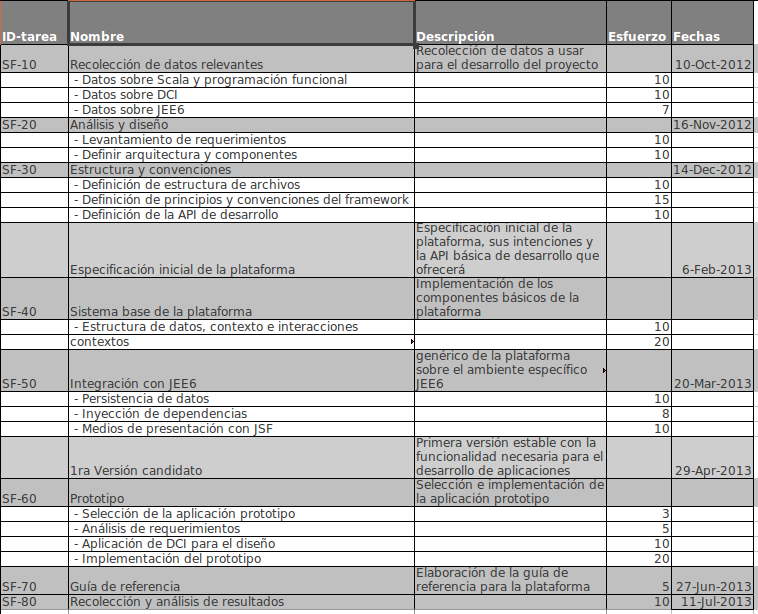
\includegraphics[width=16cm,height=13cm]{planning.png}}
	  \caption{Planificaci\'on temporal}
	\end{figure}
  \newpage


\section*{Novedad del trabajo}
\addcontentsline{toc}{section}{Novedad del trabajo}
  
  La visi\'on de una arquitectura de sistemas gen\'erica 
  puede ser aplicada a cualquier ambiente de desarrollo, 
  ya que las plataformas y herramientas usadas son detalles 
  del sistema y no definen lo que el sistema es ni lo que hace. 
  Tal arquitectura est\'a enfocada a dos aspectos importantes 
  en la industria de desarrollo, la correctitud de las aplicaciones 
  y la capacidad de las mismas de crecer y ser mantenibles. El 
  presente trabajo es un acercamiento a estos conceptos a trav\'es 
  de una herramienta de desarrollo concreta, con la cual es 
  posible elaborar sistemas cubriendo las falencias detalladas 
  en la situaci\'on problem\'atica.

\section*{Aporte del trabajo}
\addcontentsline{toc}{section}{Aporte del trabajo}
  
  El aporte del presente trabajo es tanto te\'orico como pr\'actico 
  ya que los temas en los que basa, \gls{DCI} y programaci\'on objeto-funcional, 
  son relevantes tanto para el \'area de ingenier\'ia 
  del software como para la industria de desarrollo, 
  y el artefacto resultante, una plataforma de desarrollo, 
  es una herramienta de prop\'osito
  general enfocada al desarrollo de aplicaciones reales en base 
  a las necesidades capturadas en una empresa activa en el medio. 

